As a test case to get acquainted with the PLUTO software we simulated hydrodynamic and magnetohydrodynamic blastwaves in a 2D domain.
The normalization constants for the units used are the following:
\begin{align*}
	v_0 &= 10^8 \text{cm/s}\\
	L_0 &= 10^8 \text{cm}\\
	\rho_0 &= 10^9 m_p \text{cm}^{-3}
\end{align*}
where $m_p$ is the mass of a proton. These values are of the order of what is commonly found in the solar corona. \todo{referentie naar een of andere paper}
As was noted in \cref{sec:units}, the ideal MHD equation are dimensionless.
The ideal HD equations are the ideal MHD equations without the terms relating to the magnetic field. Therefore, they are dimensionless as well.
In an effort to keep the discussion as general as possible, dimensionless quantities are used in the remainder of the section, unless explicitly stated otherwise.
In some cases, empty square brackets $[\,]$ emphasize that a quantity is dimensionless.

The initial condition for the simulations is a circle with radius $0.3$ at higher pressure $p_{in}$ than its surroundings at $p_{out} = 1$.
We ran three simulations for different values of $p_{in}$.
The first with a large pressure difference, where $p_{in} = 5$. The other two have a lower pressure difference with $p_{in} = 1.5$ and  $p_{in}=1.05$.
We use these different values of $p_{in}$ to highlight the non-linear effects on the shock wave of the case with higher pressure difference.

\subsection{Hydrodynamic shock wave}
First some technical details of the simulation.
The simulation was done on a $1024 \times 1024$ grid for a period of $t=1.5$ and an initial time step of $1e-4$.
The size of the grid is $6$ by $6$.
A snapshot of the variables describing the system was saved every $0.03$ time units, for a total of $50$ snapshots (excluding the initial condition).

\begin{figure}[H]
	%\hspace{-1cm}
	\centering
	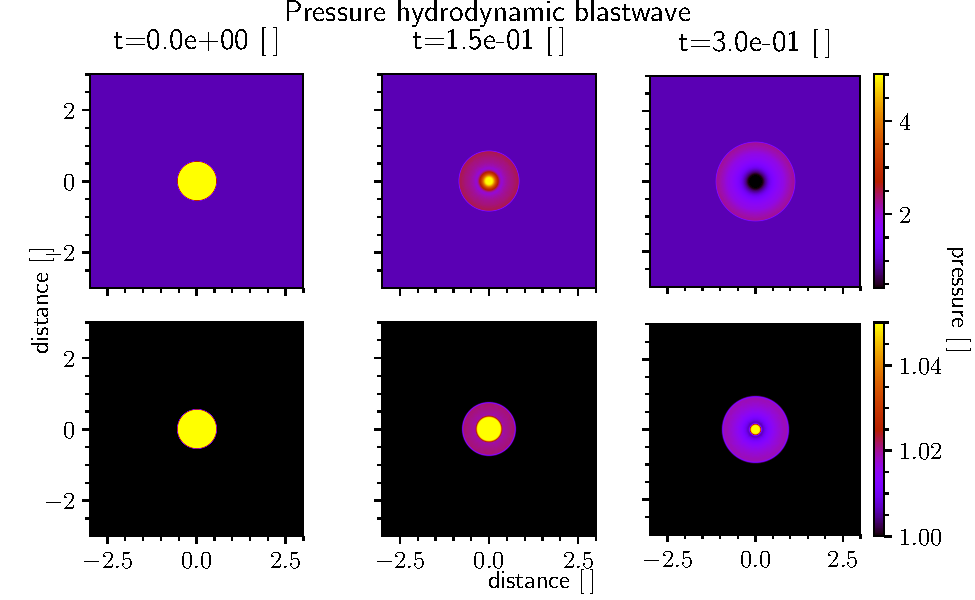
\includegraphics[width=\linewidth]{images/HD-blast-prs-1.pdf}
	\caption{Pressure profile for a blastwave in an ideal fluid at different times. The top row starts with the larger pressure difference of $5/1$, the bottom row is the blastwave with the smallest pressure difference of $1.05/1$.}
	\label{fig:HD-blast-short}
\end{figure}

In \cref{fig:HD-blast-short} the pressure profile of both scenarios is plotted for the initial condition and two frames right after the start of the simulation.
In \cref{fig:HD-blast-long} the profile is plotted for later times.
It is immediately clear that the shock wave with the higher pressure difference travels faster than the other one. However, the general shape of the wave remains the same.


In the right hand plot of \cref{fig:HD-speed} the speed of the wave front along the positive $x$-axis is plotted as a function of time. This confirms that the wave speed is lower with a lower pressure difference.
The group speed can be calculated in two ways. 
The first is to start at a point at the edge of the domain and find the first point on the line from this point to the center with a pressure higher than $1.01$ times the background pressure.
This way, we get a function $r(t,\theta)$ expressing the distance from the center to the wave front along a line as a function of the angle between this line and the $x$-axis and time.
The speed was calculated using numerical differentiation with the following central difference:
\begin{equation*}
	f'(t_0) = \frac{f(t+dt)-f(t-dt)}{2dt} + O(dt^2)
\end{equation*}
found in [REF]\todo{reference naar cursus numerieke wiskunde}. This is the simulated speed, represented by the dots.
In the left graph of \cref{fig:HD-speed}, we see that the speed is isotropic, apart from some deviations.
These deviations are mainly due to the discrete nature of the grid, which prevents calculating an exact position of the wave-front.
To mitigate this noise, the speeds calculated in all directions were averaged together to get the dots representing the wave speed in the right hand graph of \cref{fig:HD-speed}.

Using \cref{eq:Riemann-solution2} the theoretical speed of a shock in a Riemann problem was calculated, using the highest pressure in the domain as max pressure ($p_1$) and $1$ as the lowest pressure ($p_0$). This is plotted as the solid lines in \cref{fig:HD-speed}.

\begin{figure}[H]
	%\hspace{-1cm}
	\centering
	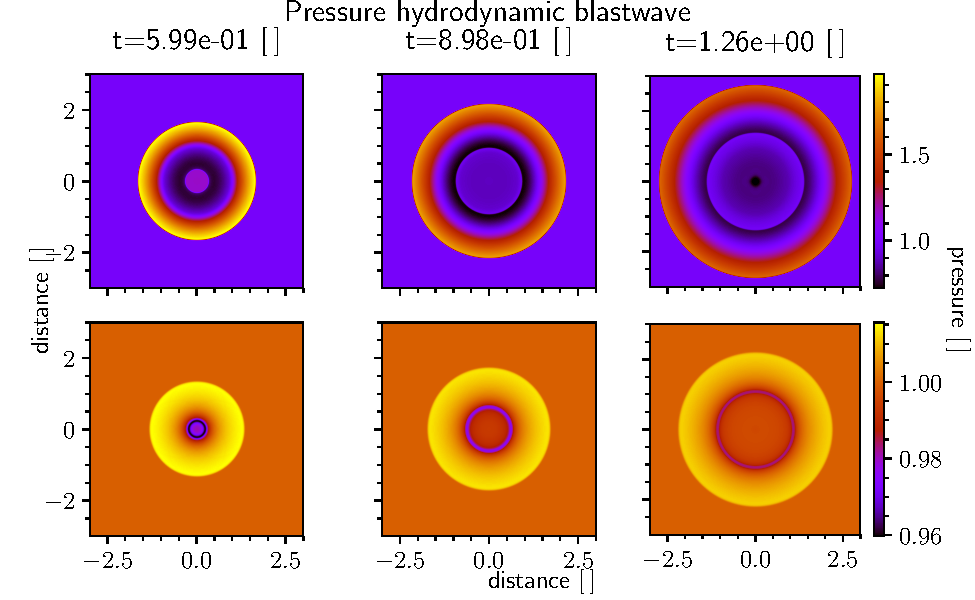
\includegraphics[width=\linewidth]{images/HD-blast-prs-2.pdf}
	\caption{Pressure profile for a blastwave in an ideal fluid at larger timescales. Initial conditions for each row are the same as in \cref{fig:HD-blast-short}.}
	\label{fig:HD-blast-long}
\end{figure}

The first 10 snapshots are not included in the right graph of \cref{fig:HD-speed}. 
The reason can be seen in \cref{fig-HD-blast-short}. 
When the shock wave starts going outwards, the pressure in the center stays at it's original pressure for some more time.
We use the max pressure in the domain to estimate $p_1$ in \cref{eq:Riemann-Solution2}. However for these first frames this is not the maximum pressure in the wave front.
It proved to be difficult to accurately detect the maximum of the wave front Therefore, the first couple of frames were left out.
The higher initial speed and sudden drop in \cref{fig:HD-speed} for $p=1.5$ is due to these effects. A closer look to the curve for $p=1.05$ will reveal something similar.

We notice that the curves do match rather closely, proving the ability of the PLUTO code to deal with shocks. 
The periodic behaviour of dots lying under and above the curve could still be an artefact of the grid discretization. However, no conclusive results were found to prove this. Thus, it could point to a systematic error.

Lastly, in \cref{fig:HD-blast-long}, there are new waves appearing from the center. This is due to the nature of a 2.5D simulation.
The initial condition has to be interpreted as a long cylinder in 3D, from which a slice perpendicular to this cylinder, is taken for the simulated. 
The secondary wave fronts can then be seen as waves coming from different points on the cylinder.

We remark that approximating the shock as a Riemann problem is a crude first-order approximation. 
The PLUTO code calculates flow velocities like this in every integration step. 
This small example highlights the importance of robust integrators and Riemann solvers, together with small enough time steps, to accurately model flow variables in the vicinity of large gradients.

\begin{figure}[H]
	%\hspace{-1cm}
	\centering
	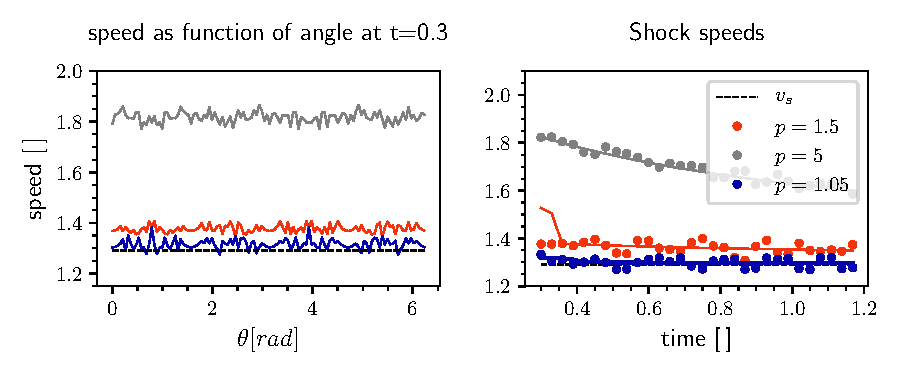
\includegraphics[width=\linewidth]{images/HD-speed.pdf}
	\caption{\emph{Left}: Speed at 3 consecutive timestamps averaged together as a function of the angle of propagation for the 3 situations. 
		The averaging was done to lower the noise and find systematic deviations.
	\emph{Right}: The speed of the wave as a function of time, along the $x$-axis. 
	The dots represent the speed calculated from the simulation data by deriving the function $x(t)$ that represents the position of the wave front. 
	The lines represent the theoretical shock speed in a Riemann-problem with as high pressure the highest pressure in the domain, and lowest pressure $1$.
	The black dashed line in both graphs is the speed of sound for linear pressure waves in a medium with pressure $1$ (code units).}
	\label{fig:HD-speed}
\end{figure}

